%Based on the code of Yiannis Lazarides
%http://tex.stackexchange.com/questions/42602/software-requirements-specification-with-latex
%http://tex.stackexchange.com/users/963/yiannis-lazarides
%Also based on the template of Karl E. Wiegers
%http://www.se.rit.edu/~emad/teaching/slides/srs_template_sep14.pdf
%http://karlwiegers.com
\documentclass{scrreprt}
\usepackage{listings}
\usepackage{underscore}
\usepackage[margin=3.0cm]{geometry}
\usepackage{enumitem}
\usepackage{graphicx,subfigure}
\usepackage[bookmarks=true]{hyperref}
\usepackage[english, spanish]{babel}
\usepackage[utf8]{inputenc}
\usepackage{float}
\usepackage{xcolor}
\usepackage{fancyhdr}
\usepackage[export]{adjustbox}
\usepackage{tabularx}
\usepackage{amsmath}
\usepackage{amsfonts}

\hypersetup{
    bookmarks=false,        % show bookmarks bar?
    pdftitle={Especificación de Requerimientos de Software},    % title
    pdfauthor={},           % author
    pdfsubject={},          % subject of the document
    pdfkeywords={},         % list of keywords
    colorlinks=true,        % false: boxed links; true: colored links
    linkcolor=blue,         % color of internal links
    citecolor=black,        % color of links to bibliography
    filecolor=black,        % color of file links
    urlcolor=purple,        % color of external links
    linktoc=page            % only page is linked
}

\def\myversion{1.0}
\date{}
\usepackage{hyperref}
\usepackage{etoolbox}

%%%%%%%%%%%
% Configurar estilo de header y footer
\fancypagestyle{plain}{
  \fancyhf{}
  \lfoot{
\includegraphics[scale=0.08,valign=c]{images/spaceLogo.png}}
  \rfoot{Pág. \thepage}
}

\pagestyle{fancy}
\fancyhf{}
\lfoot{
\includegraphics[scale=0.08,valign=c]{images/spaceLogo.png}}
\rfoot{Pág. \thepage}

\renewcommand{\headrulewidth}{0pt} % linea de header invisible
\renewcommand{\footrulewidth}{0.4pt} % linea de footer delgada

%%%%%%%%%%

\begin{document}

\setlength{\abovedisplayskip}{-10pt}
\setlength{\belowdisplayskip}{-10pt}
\setlength{\abovedisplayshortskip}{-10pt}
\setlength{\belowdisplayshortskip}{-10pt}

\begin{flushright}
	\rule{16cm}{0.2cm}\vskip1cm
    \begin{bfseries}
        \Huge{DOCUMENTO DEL \\ AVANCE \#3 (Final)}\\
        \vspace{0.5cm}
        para\\
        \vspace{0.5cm}
        Sistema de Preprocesamiento\\ y Análisis CElular\\
        \vspace{1.0cm}
        \LARGE{Versión \myversion}\\
        \vspace{1.0cm}
        Preparado por:\\ \vspace{0.5cm}
        	José Alvarado Chaves, 201129079\\
            Reggie Barker Guillén, 2014050578\\
            Joel Barrantes Garro, 2013120962\\
            Joel Schuster Valverde, 2014096796\\                        
        \vspace{1.5cm}
        Instituto Tecnológico de Costa Rica\\
        \vspace{1.5cm}
        \today\\
    \end{bfseries}
\end{flushright}


\tableofcontents


\chapter{Clases de equivalencia}

En este capítulo, se definirán las clases de equivalencia aplicables al sistema SPACE.

\section{Validez de clases}

En la siguiente tabla se especifican las clases de equivalencia, y si estas son válidas o no:

\begin{center}
    \begin{tabular}{|p{2.0cm}|p{8.0cm}|p{3.0cm}|}
        \hline
	    \textbf{Id} & \textbf{Clase de equivalencia} & \textbf{Validez} \\
        \hline
	    CE_001 & \begin{gather*} \forall x \space \in Imagen, 0\leq x \leq 255  \end{gather*} & Válida \\
        \hline
        CE_002 & 
        \begin{gather*}
        	Imagen: \left\{\space \right\}   
		\end{gather*} &   	
        Inválida \\
        \hline
        CE_003 & 
        \begin{gather*}
        	\forall x \in Groundtruth  \wedge  \forall y \in Imagen, \\
            x \in \left\{0,255\right\} \wedge  y \in \left\{0,255\right\} 				
        \end{gather*} &
        Válida \\
        \hline
        CE_004 &  \begin{gather*} Groundtruth \in \mathbb{R}^{N\times M} \wedge Imagen \in \mathbb{R}^{N\times M} 			\end{gather*}  & Válida \\
        \hline
        CE_005 & \begin{gather*} Histograma \in \mathbb{R}^{256} \end{gather*} & Válida \\
        \hline
        CE_006 & \begin{gather*} Umbral \in \mathbb{Z} \end{gather*} & Válida \\
        \hline
        CE_007 & \begin{gather*} 0 \leq Umbral \leq 255 \end{gather*} & Válida \\
        \hline
        CE_008 & \begin{gather*} FilePath: Null  \end{gather*} & Inválida \\
        \hline
        CE_009 & \begin{gather*} \parallel Files \parallel >  0  \end{gather*} & Inválida \\
        \hline
        CE_010 & \begin{gather*} ConnectionString: Null  \end{gather*} & Inválida \\
        \hline
        CE_011 & \begin{gather*} Credenciales: Null  \end{gather*} & Inválida \\
        \hline
        
	\end{tabular}
\end{center}

\section{Relación con las pruebas}

La siguiente tabla muestra relación entre las clases de equivalencia y las pruebas diseñadas:

\begin{center}
    \begin{tabular}{|p{7.0cm}|p{5.0cm}|}
        \hline
	    \textbf{Id de la clase de equivalencia} & \textbf{Id. de la prueba}\\
        \hline
        CE_001 & UN_001 \\ 
        \hline
	    CE_002 & UN_001, IT_002, UN_004 \\
        \hline
        CE_003 & UN_002 \\
        \hline
        CE_004 & UN_002 \\
        \hline
        CE_005 & UN_003 \\
        \hline
        CE_006 & UN_004 \\
        \hline
        CE_007 & UN_004 \\
        \hline
        CE_008 & IT_001, IT_002 \\
        \hline
        
        CE_009 & IT_001 \\
        \hline
        CE_010 & IT_003 \\
        \hline
        CE_011 & IT_004 \\
        \hline
    \end{tabular}
\end{center}



 \chapter{Pruebas}

En este capítulo, se especifica el diseño de las pruebas, entre las que se encuentran cuatro pruebas unitarias, cuatro de integración, y dos de sistema elaboradas con Selenium.

\section{Diseño de las pruebas}

A continuación, se definen de forma detallada las pruebas diseñadas en la siguiente tabla:

\begin{center}
    \begin{tabular}{|p{3.0cm}|p{2.2cm}|p{3.5cm}|p{2.8cm}|p{2.5cm}|}
        \hline
	    \textbf{Id. de la prueba} & \textbf{Tipo de prueba} & \textbf{Descripción} & \textbf{Precondiciones} & \textbf{Resultados esperados} \\
        \hline
        UN_001 - CentroideAreaGenTest.java & Prueba unitaria & Comprobación de que los centroides y el área de un objeto se calculan correctamente.  & Ninguna & Éxito al detectar el centroide en (50, 50) y área de 7778 píxeles \\
        \hline
        UN_002 - DiceTest.java & Prueba unitaria & Cálculo con el algoritmo de Dice para obtener la similitud entre dos imágenes binarias inversas. & Ninguna & Las imágenes coinciden en un 0\%. \\
        \hline
        UN_003 - KittlerTest.java & Prueba unitaria & Prueba de cálculo de umbral de imagen en escala de grises usando el algoritmo de Kittler. & Ninguna & El umbral $\tau$ resultante es 168. \\
        \hline
        UN_004 - UmbralizacionTest.java & Prueba unitaria & Prueba de umbralización de una imagen con un $\tau$ obtenido por Kittler. & Ninguna & Imagen binaria umbralizada, idéntica al groundtruth. \\
        \hline
        IT_001 - ImageDownloadTest.java & Prueba de integración & Prueba para verificar la descarga de una imagen existente en Mongo al disco local. & Base de datos MongoDB en ejecución & Imagen guardada con File al disco local - cellDesdeBD.png \\
        \hline
        IT_002 - ImageUploadTest.java & Prueba de integración & Prueba de subida de imagen desde disco a base de datos MongoDB & Base de datos MongoDB en ejecución & GridFSDB guardado en base de datos Mongo con éxito. \\
        \hline
        IT_003 - MySqlConnectionTest.java & Prueba de integración & Prueba de conexión simple a la base de datos MySQL & Server MySQL en ejecución & Conexión exitosa y SELECT 1 exitoso a la base de datos relacional. \\
        \hline
        IT_004 - UserValidatorTest.java & Prueba de integración & Prueba de integración entre el Validator de usuarios de Spring y Java & Spring Boot en ejecución & Validación exitosa y cero errores en la evaluación. \\
        \hline
        ST_001 - RegistrationTest.java & Prueba de sistema & Prueba de Selenium para registrar un usuario en el sistema & SPACE y MySQL en ejecución. & Mensaje de éxito al registrar el usuario \\
        \hline        
        ST_002 - UploadFailTest.java & Prueba de sistema & Prueba de restricción al tratar de crear un lote sin imágenes & Ninguna & Mensaje de restricción al crear el lote vacío.\\
        \hline
    \end{tabular}
\end{center}

\section{Evidencia de las pruebas}

Para comprobar que cada una de las pruebas se ejecuta correctamente, se adjuntan evidencias de su funcionamiento y resultados.

\subsection{Pruebas unitarias}

En esta subsección, se mostrará la evidencia del funcionamiento correcto de las cuatro pruebas unitarias, y corresponden a los algoritmos de segmentación y análisis implementados en el sistema.

\subsubsection{UN_001 - CentroideAreaGenTest.java}

\begin{figure}[H]
	\centering
    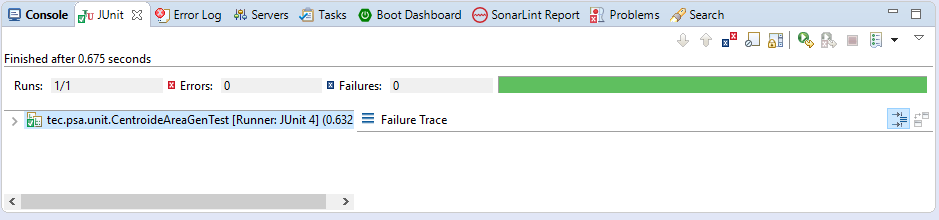
\includegraphics[width=1.0\linewidth]{images/unit/CentroideAreaGen.png}
    \caption{Resultados de ejecución de test UN_001}
\end{figure}


\subsubsection{UN_002 - DiceTest.java}

\begin{figure}[H]
	\centering
    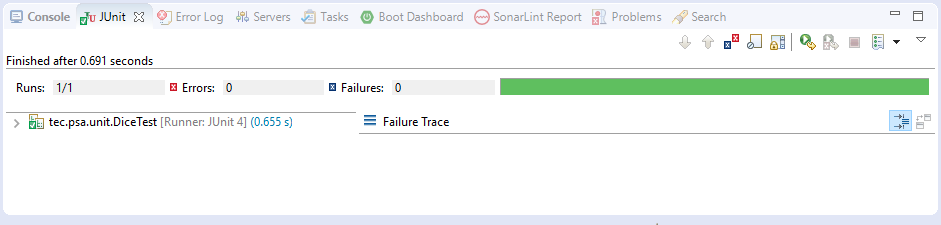
\includegraphics[width=1.0\linewidth]{images/unit/DiceTest.png}
    \caption{Resultados de ejecución de test UN_002}
\end{figure}


\subsubsection{UN_003 - KittlerTest.java}

\begin{figure}[H]
	\centering
    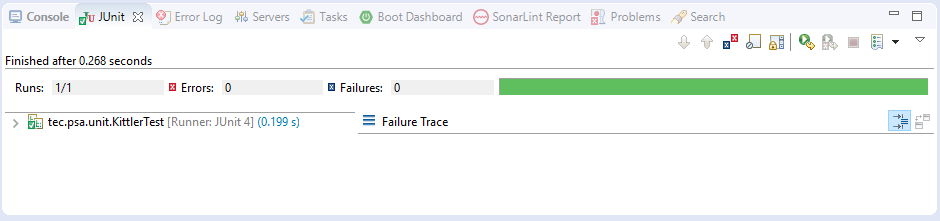
\includegraphics[width=1.0\linewidth]{images/unit/KittlerTest.png}
    \caption{Resultados de ejecución de test UN_003}
\end{figure}


\subsubsection{UN_004 - UmbralizacionTest.java}

\begin{figure}[H]
	\centering
    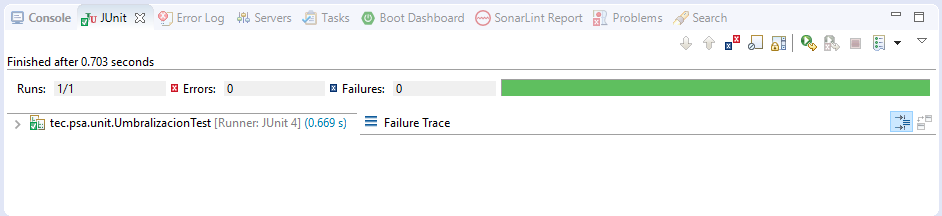
\includegraphics[width=1.0\linewidth]{images/unit/UmbralizacionTest.png}
    \caption{Resultados de ejecución de test UN_004}
\end{figure}



\subsection{Pruebas de integración}

En esta subsección, se mostrará la evidencia del funcionamiento correcto de las cuatro pruebas de integración, que corresponden a las interacciones entre los componentes que conforman el sistema, como la base de datos MongoDB, MongoDB y Java/Spring.

\subsubsection{IT_001 - ImageDownloadTest.java}

\begin{figure}[H]
	\centering
    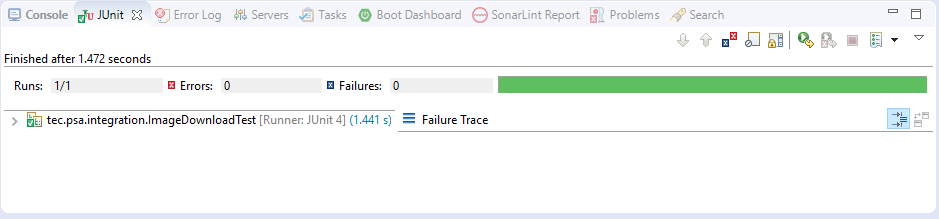
\includegraphics[width=1.0\linewidth]{images/integration/imageDownload.png}
    \caption{Resultados de ejecución de test IT_001}
\end{figure}

\begin{figure}[H]
	\centering
    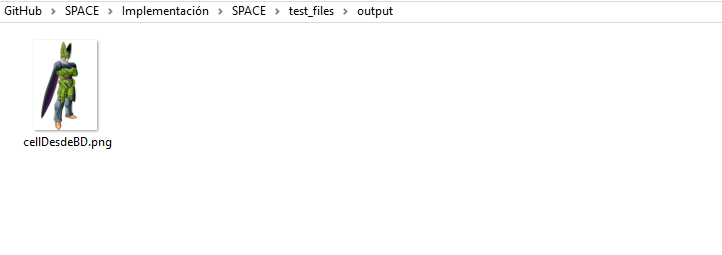
\includegraphics[width=1.0\linewidth]{images/integration/imageDownload001.png}
    \caption{Imagen descargada en el disco.}
\end{figure}

La prueba ha sido exitosa si, al navegar a la carpeta \textit{test_files/output} se observa la imagen anterior guardada localmente en el sistema de archivos.


\subsubsection{IT_002 - ImageUploadTest.java}

\begin{figure}[H]
	\centering
    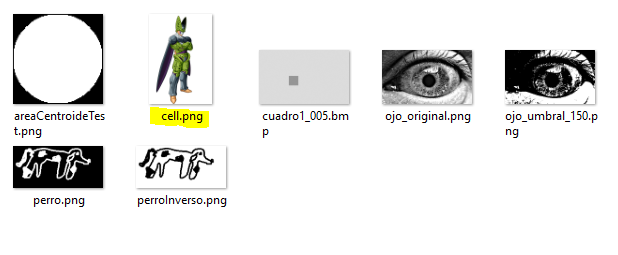
\includegraphics[width=1.0\linewidth]{images/integration/imageUpload001.png}
    \caption{Imagen a subir a la base de datos}
\end{figure}

\begin{figure}[H]
	\centering
    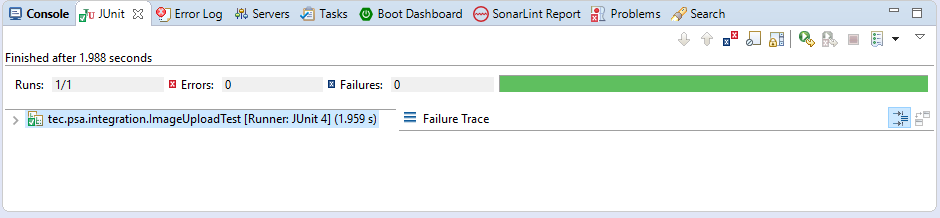
\includegraphics[width=1.0\linewidth]{images/integration/imageUpload.png}
    \caption{Resultados de ejecución de test IT_002}
\end{figure}


\subsubsection{IT_003 - MySqlConnectionTest.java}

\begin{figure}[H]
	\centering
    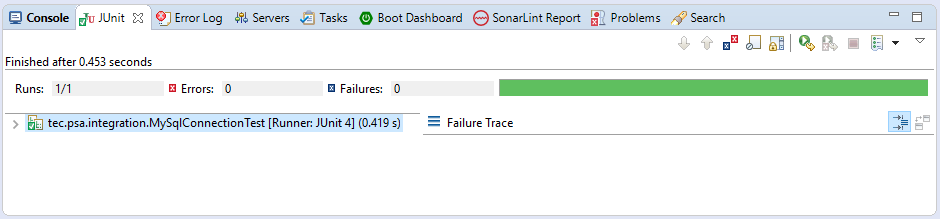
\includegraphics[width=1.0\linewidth]{images/integration/MySqlConnectionTest.png}
    \caption{Resultados de ejecución de test IT_003}
\end{figure}


\subsubsection{IT_004 - UserValidatorTest.java}

\begin{figure}[H]
	\centering
    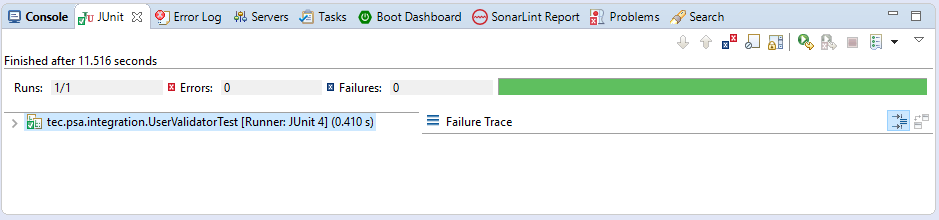
\includegraphics[width=1.0\linewidth]{images/integration/UserValidatorTest.png}
    \caption{Resultados de ejecución de test IT_004}
\end{figure}


\subsection{Pruebas de sistema}

En esta subsección, se mostrará la evidencia del funcionamiento correcto de dos pruebas de sistema, que corresponden a la usabilidad, es decir, la interacción entre un usuario y la interfaz del sistema. Se han automatizado utilizando Gecko y Selenium.

\subsubsection{ST_001 - RegistrationTest.java}

\begin{figure}[H]
	\centering
    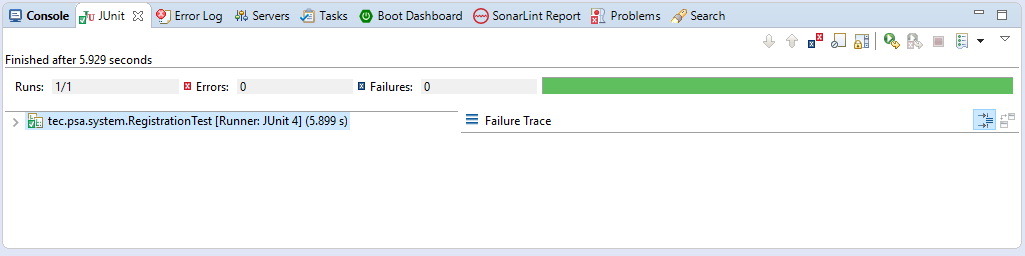
\includegraphics[width=1.0\linewidth]{images/system/registration.png}
    \caption{Resultados de ejecución de test ST_001}
\end{figure}

\subsubsection{ST_002 - UploadFailTest.java}

\begin{figure}[H]
	\centering
    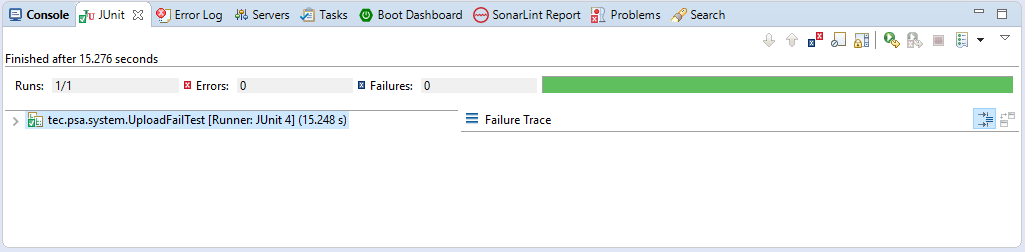
\includegraphics[width=1.0\linewidth]{images/system/uploadFail.png}
    \caption{Resultados de ejecución de test ST_002}
\end{figure}


\end{document}
